\chapter{Runtime Evaluation} % TODO: other title pls?
In this chapter we evaluate the implementation of the $DC_C$ calculus.
To do this, we extend the natural numbers program with the support of
abstract syntax of expressions.

\section{Program Definition}
\subsection{Natural Numbers}
First, we recap the implementation of the natural numbers:
\begin{align*}
&\constr{\texttt{Zero}}{x}{\epsilon}\\
&\progEnt{x}{\instOf{x}{\texttt{Zero}}}{\instOf{x}{\texttt{Nat}}}\\
&\constr{\texttt{Succ}}{x}{\instOf{x.p}{\texttt{Nat}}}\\
&\progEnt{x}{\instOf{x}{\texttt{Succ}}, \instOf{x.p}{\texttt{Nat}}}{\instOf{x}{\texttt{Nat}}}\\
&\mDecl{\texttt{prev}}{x}{\instOf{x}{\texttt{Nat}}}{\type{y}{\instOf{y}{\texttt{Nat}}}}\\
&\mImpl{\texttt{prev}}{x}{\instOf{x}{\texttt{Zero}}}{\type{y}{\instOf{y}{\texttt{Nat}}}}{x}\\
&\mImpl{\texttt{prev}}{x}{\instOf{x}{\texttt{Succ}}, \instOf{x.p}{\texttt{Nat}}}{\type{y}{\instOf{y}{\texttt{Nat}}}}{x.p}
\end{align*}
%
A natural number (\texttt{Nat}) is either the number zero (\texttt{Zero})
or a successor of a natural number (\texttt{Succ}).
\texttt{Succ} has a field $p$ of class \texttt{Nat}.
The function \texttt{prev} computes the previous element of a natural number.
The previous number of zero is defined as zero.
We changed the implementation for this case.
The program defined in \Cref{ex:dcc-naturalnumbers} created a new
instance of class \texttt{Zero}.
The new implementation returns the parameter,
as it is constrained to be an instance of \texttt{Zero}.

\subsection{Numeric Expressions}
We define a program for the abstract syntax of numeric expressions:
%
\begin{align*}
&\constr{\texttt{Lit}}{x}{\instOf{x.value}{\texttt{Nat}}}\\
&\progEnt{x}{\instOf{x}{\texttt{Lit}}, \instOf{x.value}{\texttt{Nat}}}{\instOf{x}{\texttt{Exp}}}\\
&\constr{\texttt{Plus}}{x}{\instOf{x.l}{\texttt{Exp}}, \instOf{x.r}{\texttt{Exp}}}\\
&\progEnt{x}{\instOf{x}{\texttt{Plus}}, \instOf{x.l}{\texttt{Exp}}, \instOf{x.r}{\texttt{Exp}}}{\instOf{x}{\texttt{Exp}}}
\end{align*}
%
The constructor \texttt{Lit} defines a field \mIt{value},
representing numeric literals with the value \mIt{value}.
The constructor \texttt{Plus} defines fields $l$ and $r$,
representing the addition of $r$ and $l$.
The two constraint entailment declarations express
the inheritance relation of
\texttt{Lit} and \texttt{Plus} to \texttt{Exp}.

\begin{figure}[h]
\begin{center}
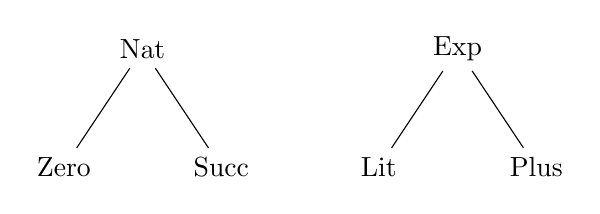
\begin{tikzpicture}
  \node (Nat) at (-1,0) {Nat};
  \node (Zero) at (-2,-1.5) {Zero};
  \node (Succ) at (0,-1.5) {Succ};
  \path (Nat) edge (Zero);
  \path (Nat) edge (Succ);
  
  \node (Exp) at (3,0) {Exp};
  \node (Lit) at (2,-1.5) {Lit};
  \node (Plus) at (4,-1.5) {Plus};
  \path (Exp) edge (Lit);
  \path (Exp) edge (Plus);
% \node (comment) at (-0.5, -0.5) {asdf};
\end{tikzpicture}
\end{center}
\caption{Inheritance Relation}
\label{fig:aexp-inheritance}
\end{figure}\quad\\
\Cref{fig:aexp-inheritance} shows the
inheritance relation of the natural numbers
and the numeric expressions.

\subsection{Numeric Expression Evaluation}
We extend the abstract syntax of numeric expressions
with a method to evaluate expressions:
%
\begin{align*}
&\mDecl{\texttt{eval}}{x}{\instOf{x}{\texttt{Exp}}}{\type{y}{\instOf{y}{\texttt{Exp}}}}\\
&\mImpl{\texttt{eval}}
       {x}
       {\instOf{x}{\texttt{Lit}}, \instOf{x.value}{\texttt{Nat}}}
       {\type{y}{\instOf{y}{\texttt{Exp}}}}
       {x}\\
%&\mImpl{\texttt{eval}}
%       {x}
%       {\instOf{x}{\texttt{Plus}},
%        \instOf{x.l}{\texttt{Lit}},
%        \instOf{x.r}{\texttt{Lit}},
%        \instOf{x.l.value}{\texttt{Nat}},
%        \instOf{x.r.value}{\texttt{Zero}}}
%       {\type{y}{\instOf{y}{\texttt{Exp}}}}
%       {x.l}\\
&\texttt{eval}(x. \instOf{x}{\texttt{Plus}},
                  \instOf{x.l}{\texttt{Lit}},
                  \instOf{x.r}{\texttt{Lit}},
                  \instOf{x.l.value}{\texttt{Nat}},\\
&\qquad\qquad\qquad\qquad\qquad
                  \instOf{x.r.value}{\texttt{Zero}} )
    : \type{y}{\instOf{y}{\texttt{Exp}}} := \\
&\quad x.l\\
%&\mImpl{\texttt{eval}}
%       {x}
%       {\instOf{x}{\texttt{Plus}},
%        \instOf{x.l}{\texttt{Lit}},
%        \instOf{x.r}{\texttt{Lit}},
%        \instOf{x.l.value}{\texttt{Nat}},
%        \instOf{x.r.value}{\texttt{Succ}},
%        \instOf{x.r.value.p}{\texttt{Nat}}}
%       {\type{y}{\instOf{y}{\texttt{Exp}}}}{}\\
%         &\quad\texttt{eval}(
%           \new \texttt{Plus}(\\
%             &\qquad\pathEq{l}{
%               \objConstr{\texttt{Lit}}
%                         {\pathEq{value}{ \objConstr{\texttt{Succ}}{\pathEq{p}{x.l.value}}}}},\\
%             &\qquad\pathEq{r}{
%               \objConstr{\texttt{Lit}}
%                         {\pathEq{value}{\texttt{prev}(x.r.\mIt{value})}}}
%           )
%         )\\
&\texttt{eval}(x. \instOf{x}{\texttt{Plus}},
                  \instOf{x.l}{\texttt{Lit}},
                  \instOf{x.r}{\texttt{Lit}},
                  \instOf{x.l.value}{\texttt{Nat}},\\
&\qquad\qquad
                  \instOf{x.r.value}{\texttt{Succ}},
                  \instOf{x.r.value.p}{\texttt{Nat}}
              ): \type{y}{\instOf{y}{\texttt{Exp}}} :=\\
&\quad\texttt{eval}(
           \new \texttt{Plus}(\\
             &\qquad\pathEq{l}{
               \objConstr{\texttt{Lit}}
                         {\pathEq{value}{ \objConstr{\texttt{Succ}}{\pathEq{p}{x.l.value}}}}},\\
             &\qquad\pathEq{r}{
               \objConstr{\texttt{Lit}}
                         {\pathEq{value}{\texttt{prev}(x.r.\mIt{value})}}}
           )
         )\\
&\mImpl{\texttt{eval}}
       {x}
       {\instOf{x}{\texttt{Plus}},
        \instOf{x.l}{\texttt{Exp}},
        \instOf{x.r}{\texttt{Plus}},
        \instOf{x.r.l}{\texttt{Exp}},
        \instOf{x.r.r}{\texttt{Exp}}}
       {\type{y}{\instOf{y}{\texttt{Exp}}}}{}\\
       &\quad\texttt{eval}(
         \objConstr{\texttt{Plus}}
                   {
                     \pathEq{l}{x.l},
                     \pathEq{r}{\texttt{eval(x.r)}}
                   }
       )\\
&\mImpl{\texttt{eval}}
       {x}
       {\instOf{x}{\texttt{Plus}},
        \instOf{x.l}{\texttt{Plus}},
        \instOf{x.r}{\texttt{Exp}},
        \instOf{x.l.l}{\texttt{Exp}},
        \instOf{x.l.r}{\texttt{Exp}}}
       {\type{y}{\instOf{y}{\texttt{Exp}}}}{}\\
       &\quad\texttt{eval}(
         \objConstr{\texttt{Plus}}
                   {
                     \pathEq{l}{\texttt{eval(x.l)}},
                     \pathEq{r}{x.r}
                   }
       )
\end{align*}
We abstractly declare method \texttt{eval}
to evaluate an expression to an expression,
where literals are the values of the expression language.
We use the constraints on the parameter to
model a behavior similar to pattern matching.
We overload the method for each case
we want to match and set the requirements
on the parameter accordingly.

\subsubsection{Literals}
Since literals are considered to be values,
we evaluate an input $x$ conforming to the requirements
\instOf{x}{\texttt{Lit}} and \instOf{x.value}{\texttt{Nat}} to itself.
The requirements make sure that the input is a proper literal.

\subsubsection{Addition}
We implement the evaluation of \texttt{Plus} expressions
through evaluation on the right-hand side.
We consider four cases:
\begin{enumerate}
  \item Fields $l$ and $r$ are literals and $r$ contains the \mIt{value} \texttt{Zero}.
  \item Fields $l$ and $r$ are literals and $r$ contains a \mIt{value} \texttt{Succ}.
  \item Field $r$ is a \texttt{Plus} expression.
  \item Field $l$ is a \texttt{Plus} expression.
\end{enumerate}
%
The implementation of these cases is as follows:
\paragraph{1.}
The parameter is a \texttt{Plus} expression,
both fields are literals and $r.\mIt{value}$ is \texttt{Zero}.
The result of the evaluation is $l$.

\paragraph{2.}
The parameter $x$ is a \texttt{Plus} expression,
both fields are literals and $x.r.\mIt{value}$ contains a \texttt{Succ}.
We create a new \texttt{Plus}.
We set $l$ to be the successor of $x.l$
and $r$ to be the previous number of $x.r$.

\paragraph{3. and 4.}
The parameter $x$ is a \texttt{Plus} expression
and $x.l$ or $x.r$ are \texttt{Plus} expressions.
We propagate evaluation to $x.l$ or $x.r$ respectively.

\section{Object Construction}
\label{sec:time-out}
We interpret expressions of the defined program.
We set the time out of the solver to $2$ seconds.

We construct literals capturing $0$ and $1$.
\begin{align*}
  (h_0, \mIt{zero}) &:= \mIt{interp}(\epsilon, \newInstNoArgs{\texttt{Zero}})\\
  (h_{l0}, \mIt{litZero}) &:= \mIt{interp}(h_0, \newInst{\texttt{Lit}}{\mIt{value}}{\mIt{zero}})\\
  (h_1, \mIt{one}) &:= \mIt{interp}(h_{l0}, \newInst{\texttt{Succ}}{p}{\mIt{zero}})\\
  (h_{l1}, \mIt{litOne}) &:= \mIt{interp}(h_1, \newInst{\texttt{Lit}}{\mIt{value}}{\mIt{one}})
\end{align*}
We obtain
\begin{align*}
h_{l1} = &x_1 \mapsto (\texttt{Zero}, \epsilon)\\
         &x_2 \mapsto (\texttt{Lit}, [\pathEq{\mIt{value}}{x_1}])\\
         &x_3 \mapsto (\texttt{Succ}, [\pathEq{\mIt{p}}{x_1}])
\end{align*}
and $litOne = \newInst{\texttt{Lit}}{\mIt{value}}{\mIt{x_3}}$.
We observe that the last call to the interpreter
returned prematurely.
By inspecting the steps taken by the interpreter, we find that
the entailment
\[
  \entails{
            \instBy{x_1}{\texttt{Zero}},
            \instBy{x_3}{\texttt{Succ}},
            \pathEq{x_3.p}{x_1},
            \instBy{x_4}{\texttt{Lit}},
            \pathEq{x_4.value}{x_3}
          }
          {\instOf{x_4.value}{\texttt{Nat}}}
\]
could not be shown by the solver.
We know that
\begin{align*}
\entails
  {
    \instOf{x_3}{\texttt{Succ}},
    \instOf{x_3.p}{\texttt{Nat}}
  }
  {&\instOf{x_3}{\texttt{Nat}}}\\
\entails
  {\instOf{x_1}{\texttt{Zero}}}
  {&\instOf{x_1}{\texttt{Nat}}}\\
\entails
  {\pathEq{x_4.value}{x_3},
   \instOf{x_3}{\texttt{Nat}}}
  {&\instOf{x_4.value}{\texttt{Nat}}}
\end{align*}
can be shown by the solver.
These are sub-goals of the timed out derivation.

\section{Optimization}
We observed in \Cref{sec:time-out}
that the solver could not show an entailment,
despite being able to show the subgoals of the entailment
in isolation.
We can pre optimize the entailment to be shown,
to help the solver find a derivation.

\subsection{Apply Path-Equivalence}
\begin{figure}[h]
\begin{lstlisting}
private def preprocEquiv(
               cs: List[Constraint]): List[Constraint] = {
  val eqs = cs.filter {
    case PathEquivalence(_, _) => true case _ => false
  }
  var res = cs
  eqs.foreach {
    case PathEquivalence(x@Id(_), p) =>
      res = res.map(c => substitute(x, p, c))
    case PathEquivalence(p, x@Id(_)) =>
      res = res.map(c => substitute(x, p, c))
    case _ => ()
  }
  res.filter {
    case PathEquivalence(p, q) if p == q => false
    case _ => true
  }
}
\end{lstlisting}
\end{figure}

\subsection{Explore Inheritance}

\begin{figure}[h]
\begin{lstlisting}
private def preprocInheritance(
         cs: List[Constraint]): List[Constraint] = {
  val insts = cs.filter {
    case InstanceOf(_, _) => true case _ => false
  }
  var res = cs
  insts.foreach {
    case InstanceOf(x, _) =>
      classes.foreach {
        case cls1
        if entails(cs, InstanceOf(x, cls1), List()) =>
          res = InstanceOf(x, cls1) :: res
        case _ => ()
      }
    case _ => ()
  }
  res
}
\end{lstlisting}
\end{figure}

%%% Local Variables: 
%%% mode: latex
%%% TeX-master: "../thesis"
%%% End: 
